\documentclass{article}
\usepackage{amsmath, enumitem}
\usepackage{graphicx}
\usepackage{booktabs}
\usepackage{tabularx}
\usepackage[margin=1in]{geometry}
\usepackage{float}
\restylefloat{table}
\usepackage{placeins}
\usepackage{listings}

\usepackage{color}
 
\definecolor{codegreen}{rgb}{0,0.6,0}
\definecolor{codegray}{rgb}{0.5,0.5,0.5}
\definecolor{codepurple}{rgb}{0.58,0,0.82}
\definecolor{backcolour}{rgb}{0.95,0.95,0.92}
 
\lstdefinestyle{mystyle}{
    backgroundcolor=\color{backcolour},   
    commentstyle=\color{codegreen},
    keywordstyle=\color{magenta},
    numberstyle=\tiny\color{codegray},
    stringstyle=\color{codepurple},
    basicstyle=\footnotesize,
    breakatwhitespace=false,         
    breaklines=true,                 
    captionpos=b,                    
    keepspaces=true,                 
    numbers=left,                    
    numbersep=5pt,                  
    showspaces=false,                
    showstringspaces=false,
    showtabs=false,                  
    tabsize=2
}

\lstset{style=mystyle}

\begin{document}

\title{Econ 758 Homework 1}
\author{Ege Can, John Appert}
\maketitle

\section{Question 1}

\begin{enumerate}[label=\alph*]
\item Give a short description of the relevant aspects of the EITC expansion in 1993.(Hint: Have a look at Eissa and Hoynes, 2004.) Briefly discuss the theoretical predictions for the impact of the reform on the labor market participation of  single women with children. You do  not need  to present a formal model !

\item Would you expect the number of children to influence the size of the effect Why or why not? Explain.


\item  Generate a table with descriptive statistics (Table 1, structured as i
n Table I in Eissa and Liebman, 1996), which contains the sample means of the variables nonwhite age ed work  earn  for  two groups: single women with and without children. You do not need to display the  standard deviations. Briefly discuss the differences.

\item  Now calculate the sample means separately for single women with one child and women with two or m?ore children (add the information to Table 1). How do they differ from each other

\end{enumerate}

\section{Question 2}

For the following analysis you need to generate two dummy variables to identify the treatment group (single women with children) [call it child] and the post-treatment period (1994-1996) [call it post1993].

\begin{enumerate}[label=\alph*]
\item  Create a figure (Figure 1) that illustrates the annual mean labor market participation rates by year (1991-1996) for single women with children (treatment group) and single women without children (control group).Label the axes and include a title and a legend into the graph.


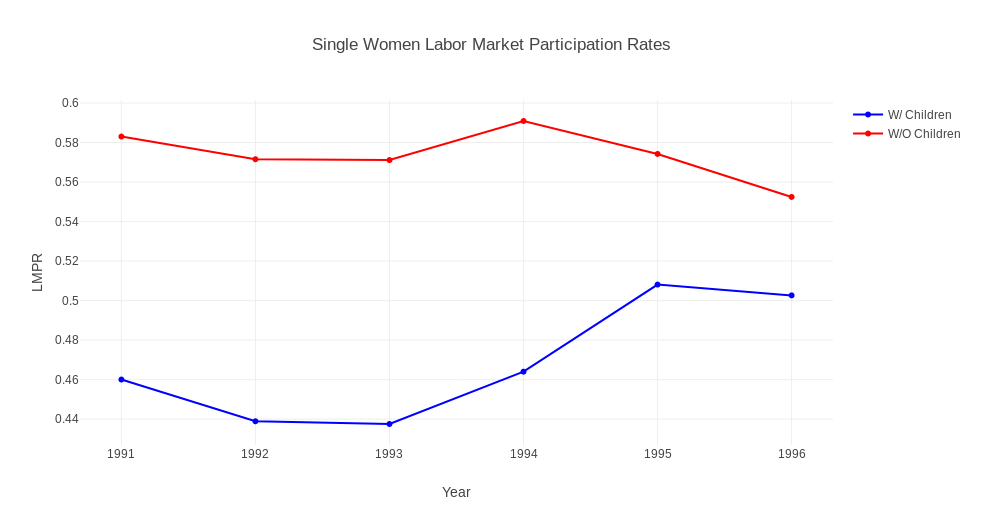
\includegraphics[width=5in, height=3in]{newplot}



\item Now normalize the value of the labor force participation rate for each of the two groups to group-specific 1991 values. That is, the mean of the labor  market participation rates in 1991 become equal to 1. Plot a graph (as the one before, including labeling, title, and legend) in Figure 2.



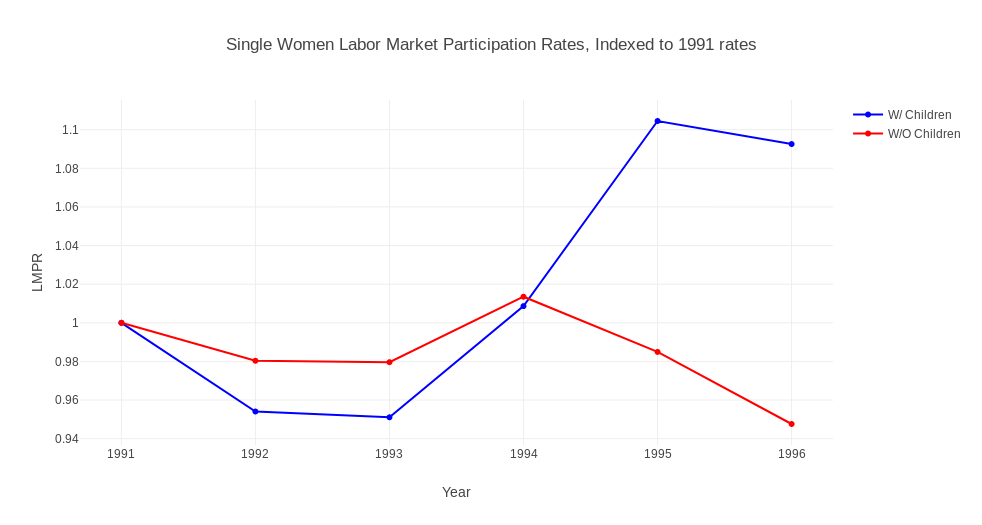
\includegraphics[width=5in, height=3in]{figure2}




\item  Based on Figures 1 and 2, discuss the validity of using single women without children as control group.

When looking at figure one it is difficult to determine whether or not the idea of using single women without children as a control group is valid.  The levels of labor market participation are significantly different and both trends seem similar.  However, once we index the labor market participation rate to 1991 and look at changes in the level with respect to 1991 we see that both groups track closely until 1993 when there is a divergence.  This implies that we can use single woment without children as a control group.

\item Calculate the sample means of labor force participation rates (work) of women with and without children for the pre-(average over 1991-1993) and post-reform (average over 1994-1996) period. Organize your table (Table 2) as in Table II in Eissa and Liebman (1996).

TODO:  Insert table from notebook.

\item Calculate the within-and between-group differences as well as the unconditional difference-in-differences estimate and add them to Table 2. Briefly comment on your results.

\item  Repeat the comparison separately for women with one child and for women with at least two children for the years before and after the EITC expansion. Again compute the within-and between-group differences and the difference-in-differences estimates. Compare each of the two groups separately to single women without children (the control group). Display the results in Table 3 and discuss your findings. For which of the two groups do you find larger treatment effects? Is this consistent with the theoretical predictions?

\item Return to the comparison of women with and without children. Estimate the difference-in-differences effect from the EITC expansion by running OLS regressions. As dependent variable, use the dummy indicating labor market participation(work). First run a regression without controls (“unconditional diff-in-diff estimate”). Then add control variables (urate nonwhite age ed) to obtain the “conditional diff-in-diff estimate”. Present your results (including standard errors) in Table 4 and interpret them. Compare the estimates and their statistical significance for the conditional and unconditional difference-in-differences estimates. Also comment on the estimated coefficients of child and post1993.

\begin{center}
\begin{tabular}{lclc}
\toprule
\textbf{Dep. Variable:}    &       work       & \textbf{  R-squared:         } &     0.013   \\
\textbf{Model:}            &       OLS        & \textbf{  Adj. R-squared:    } &     0.012   \\
\textbf{Method:}           &  Least Squares   & \textbf{  F-statistic:       } &     58.45   \\
\textbf{Date:}             & Wed, 20 Feb 2019 & \textbf{  Prob (F-statistic):} &  1.54e-37   \\
\textbf{Time:}             &     08:01:06     & \textbf{  Log-Likelihood:    } &   -9884.9   \\
\textbf{No. Observations:} &       13746      & \textbf{  AIC:               } & 1.978e+04   \\
\textbf{Df Residuals:}     &       13742      & \textbf{  BIC:               } & 1.981e+04   \\
\textbf{Df Model:}         &           3      & \textbf{                     } &             \\
\bottomrule
\end{tabular}
\begin{tabular}{lcccccc}
                  & \textbf{coef} & \textbf{std err} & \textbf{t} & \textbf{P$>$$|$t$|$} & \textbf{[0.025} & \textbf{0.975]}  \\
\midrule
\textbf{const}    &       0.5755  &        0.009     &    65.060  &         0.000        &        0.558    &        0.593     \\
\textbf{parent}   &      -0.1295  &        0.012     &   -11.091  &         0.000        &       -0.152    &       -0.107     \\
\textbf{Post1993} &      -0.0021  &        0.013     &    -0.160  &         0.873        &       -0.027    &        0.023     \\
\textbf{interact} &       0.0469  &        0.017     &     2.732  &         0.006        &        0.013    &        0.081     \\
\bottomrule
\end{tabular}
\begin{tabular}{lclc}
\textbf{Omnibus:}       &  5.965 & \textbf{  Durbin-Watson:     } &    1.934  \\
\textbf{Prob(Omnibus):} &  0.051 & \textbf{  Jarque-Bera (JB):  } & 2175.929  \\
\textbf{Skew:}          & -0.051 & \textbf{  Prob(JB):          } &     0.00  \\
\textbf{Kurtosis:}      &  1.054 & \textbf{  Cond. No.          } &     7.14  \\
\bottomrule
\end{tabular}
%\caption{OLS Regression Results}
\end{center}

Warnings: \newline
 [1] Standard Errors assume that the covariance matrix of the errors is correctly specified.

\begin{center}
\begin{tabular}{lclc}
\toprule
\textbf{Dep. Variable:}    &       work       & \textbf{  R-squared:         } &     0.027   \\
\textbf{Model:}            &       OLS        & \textbf{  Adj. R-squared:    } &     0.027   \\
\textbf{Method:}           &  Least Squares   & \textbf{  F-statistic:       } &     55.09   \\
\textbf{Date:}             & Wed, 20 Feb 2019 & \textbf{  Prob (F-statistic):} &  3.84e-78   \\
\textbf{Time:}             &     08:04:28     & \textbf{  Log-Likelihood:    } &   -9781.8   \\
\textbf{No. Observations:} &       13746      & \textbf{  AIC:               } & 1.958e+04   \\
\textbf{Df Residuals:}     &       13738      & \textbf{  BIC:               } & 1.964e+04   \\
\textbf{Df Model:}         &           7      & \textbf{                     } &             \\
\bottomrule
\end{tabular}
\begin{tabular}{lcccccc}
                  & \textbf{coef} & \textbf{std err} & \textbf{t} & \textbf{P$>$$|$t$|$} & \textbf{[0.025} & \textbf{0.975]}  \\
\midrule
\textbf{const}    &       0.4959  &        0.036     &    13.960  &         0.000        &        0.426    &        0.565     \\
\textbf{parent}   &      -0.1179  &        0.012     &    -9.891  &         0.000        &       -0.141    &       -0.095     \\
\textbf{Post1993} &      -0.0234  &        0.014     &    -1.730  &         0.084        &       -0.050    &        0.003     \\
\textbf{urate}    &      -0.0164  &        0.003     &    -4.962  &         0.000        &       -0.023    &       -0.010     \\
\textbf{nonwhite} &      -0.0445  &        0.009     &    -4.945  &         0.000        &       -0.062    &       -0.027     \\
\textbf{age}      &       0.0020  &        0.000     &     4.466  &         0.000        &        0.001    &        0.003     \\
\textbf{ed}       &       0.0171  &        0.002     &    10.477  &         0.000        &        0.014    &        0.020     \\
\textbf{interact} &       0.0495  &        0.017     &     2.905  &         0.004        &        0.016    &        0.083     \\
\bottomrule
\end{tabular}
\begin{tabular}{lclc}
\textbf{Omnibus:}       &  4.872 & \textbf{  Durbin-Watson:     } &    1.939  \\
\textbf{Prob(Omnibus):} &  0.088 & \textbf{  Jarque-Bera (JB):  } & 2046.360  \\
\textbf{Skew:}          & -0.046 & \textbf{  Prob(JB):          } &     0.00  \\
\textbf{Kurtosis:}      &  1.112 & \textbf{  Cond. No.          } &     330.  \\
\bottomrule
\end{tabular}
%\caption{OLS Regression Results}
\end{center}

Warnings: \newline
 [1] Standard Errors assume that the covariance matrix of the errors is correctly specified.


\item Estimate a conditional (i.e., including urate nonwhite age ed), “placebo” treatment model on the pre-treatment period. For this purpose, take data from the years 1991-1993 only and leave the treatment and control groups unchanged. Assume for the analysis that the placebo reform would have taken place on January 1st, 1992 (generate a dummy variable postplacebo that is one for year 1992 and after and an interaction with child) and present your results (including standard errors) in Table 5. What do you find?

\begin{center}
\begin{tabular}{lclc}
\toprule
\textbf{Dep. Variable:}    &       work       & \textbf{  R-squared:         } &     0.031   \\
\textbf{Model:}            &       OLS        & \textbf{  Adj. R-squared:    } &     0.030   \\
\textbf{Method:}           &  Least Squares   & \textbf{  F-statistic:       } &     34.06   \\
\textbf{Date:}             & Wed, 20 Feb 2019 & \textbf{  Prob (F-statistic):} &  4.84e-47   \\
\textbf{Time:}             &     08:05:32     & \textbf{  Log-Likelihood:    } &   -5254.1   \\
\textbf{No. Observations:} &        7401      & \textbf{  AIC:               } & 1.052e+04   \\
\textbf{Df Residuals:}     &        7393      & \textbf{  BIC:               } & 1.058e+04   \\
\textbf{Df Model:}         &           7      & \textbf{                     } &             \\
\bottomrule
\end{tabular}
\begin{tabular}{lcccccc}
                  & \textbf{coef} & \textbf{std err} & \textbf{t} & \textbf{P$>$$|$t$|$} & \textbf{[0.025} & \textbf{0.975]}  \\
\midrule
\textbf{const}    &       0.5403  &        0.048     &    11.281  &         0.000        &        0.446    &        0.634     \\
\textbf{parent}   &      -0.1092  &        0.020     &    -5.490  &         0.000        &       -0.148    &       -0.070     \\
\textbf{Post1992} &      -0.0002  &        0.018     &    -0.009  &         0.993        &       -0.036    &        0.036     \\
\textbf{urate}    &      -0.0210  &        0.004     &    -4.750  &         0.000        &       -0.030    &       -0.012     \\
\textbf{nonwhite} &      -0.0394  &        0.012     &    -3.265  &         0.001        &       -0.063    &       -0.016     \\
\textbf{age}      &       0.0019  &        0.001     &     3.237  &         0.001        &        0.001    &        0.003     \\
\textbf{ed}       &       0.0157  &        0.002     &     7.103  &         0.000        &        0.011    &        0.020     \\
\textbf{interact} &      -0.0127  &        0.024     &    -0.525  &         0.599        &       -0.060    &        0.035     \\
\bottomrule
\end{tabular}
\begin{tabular}{lclc}
\textbf{Omnibus:}       &  0.010 & \textbf{  Durbin-Watson:     } &     1.968  \\
\textbf{Prob(Omnibus):} &  0.995 & \textbf{  Jarque-Bera (JB):  } &  1083.431  \\
\textbf{Skew:}          &  0.003 & \textbf{  Prob(JB):          } & 5.44e-236  \\
\textbf{Kurtosis:}      &  1.126 & \textbf{  Cond. No.          } &      328.  \\
\bottomrule
\end{tabular}
%\caption{OLS Regression Results}
\end{center}

Warnings: \newline
 [1] Standard Errors assume that the covariance matrix of the errors is correctly specified.

​



\end{enumerate}


\section{Code}

\begin{lstlisting}[language=Python]
import pandas as pd
import numpy as np

#import data visualization library
import plotly.plotly as py
import plotly.graph_objs as go
from plotly.offline import download_plotlyjs, init_notebook_mode, plot, iplot

#suppress warnings
import warnings
warnings.simplefilter("ignore")

#regression
import statsmodels.api as sm

#Read in the data
df=pd.read_stata('ps1.dta')

#Initial data munging

df['employed']=np.where(df['work']==1,1,0)
df['unemployed']=np.where(df['work']==0,1,0)
df['parent']=np.where(df['children']!=0,1,0)

#pivot by year and parent and then reset the index
df1=df.groupby(['year', 'parent']).sum()
df1=df1.reset_index()

#calculate the lfpr for both parents and no parents
df1['urate']=(df1['employed'])/(df1['employed']+df1['unemployed'])
parent=df1[df1['parent']==1]
nparent=df1[df1['parent']==0]

#Generate figure 1
# Add data
year = parent['year']
parentLMPR= parent['urate']
nparentLMPR = nparent['urate']


# Create and style traces
trace0 = go.Scatter(
    x = year,
    y = parentLMPR,
    name = 'W/ Children',
    line = dict(
        color = ('blue'),
        width = 2)
)
trace1 = go.Scatter(
    x = year,
    y = nparentLMPR,
    name = 'W/O Children',
    line = dict(
        color = ('red'),
        width = 2,)
)


data = [trace0, trace1]

# Edit the layout
layout = dict(title = 'Single Women Labor Market Participation Rates',
              xaxis = dict(title = 'Year'),
              yaxis = dict(title = 'LMPR'),
              )

fig = dict(data=data, layout=layout)
py.iplot(fig, filename='raw-plot')

#Reindexing to 1991
pBaseLevel=parent.iloc[0,3]
nBaseLevel=nparent.iloc[0,3]
parent['index']=parent['urate']/pBaseLevel
nparent['index']=nparent['urate']/nBaseLevel

#Generate figure 2
# Add data
year = parent['year']
piLMPR= parent['index']
niLMPR = nparent['index']


# Create and style traces
trace0 = go.Scatter(
    x = year,
    y = piLMPR,
    name = 'W/ Children',
    line = dict(
        color = ('blue'),
        width = 2)
)
trace1 = go.Scatter(
    x = year,
    y = niLMPR,
    name = 'W/O Children',
    line = dict(
        color = ('red'),
        width = 2,)
)


data = [trace0, trace1]

# Edit the layout
layout = dict(title = 'Single Women Labor Market 
			   Participation Rates, Indexed to 1991 rates',
              xaxis = dict(title = 'Year'),
              yaxis = dict(title = 'LMPR'),
              )

fig = dict(data=data, layout=layout)
py.iplot(fig, filename='index-plot')

#Calculating diff-in-diff
parent=df[df['parent']==1]
nparent=df[df['parent']!=1]

#calculate the average of the treatment group pre-1994
tc1=parent[parent['year']<1994]
tc1_empl=tc1['work'].sum()
tc1_mean=tc1_empl/len(tc1)

#calculate the average of the treatment group post-1994
tc2=parent[parent['year']>1993]
tc2_empl=tc2['work'].sum()
tc2_mean=tc2_empl/len(tc2)

#calculate the average of the control group pre-1994
cg1=nparent[nparent['year']<1994]
cg1_empl=cg1['work'].sum()
cg1_mean=cg1_empl/len(cg1)

#calculate the average of the control group post-1994
cg2=nparent[nparent['year']>1993]
cg2_empl=cg2['work'].sum()
cg2_mean=cg2_empl/len(cg2)

#calculate diffs
dif1=tc2_mean-tc1_mean
dif2=cg2_mean-cg1_mean
dif_dif=dif1-dif2

#print (tc1_mean, tc2_mean, cg1_mean, cg2_mean)

l1=["Treatment Group", len(parent), tc1_mean, tc2_mean, dif1, '']
l2=["Control Group", len(nparent), cg1_mean, cg2_mean, dif2, dif_dif]

table=[l1, l2]

headers=['Group', 'Sample Size', 'Pre-1993', 
		'Post-1993', 'Difference', 'Difference-in-differences']

table2=pd.DataFrame(table, columns=headers)

#table2

#diff-in-diff w/ one child and two children

one_child=df[df['children']==1]
two_child=df[df['children']>1]

#calculate the average of the treatment group with one child pre-1994
tg1c1=one_child[one_child['year']<1994]
tg1c1_empl=tg1c1['work'].sum()
tg1c1_mean=tg1c1_empl/len(tg1c1)

#calculate the average of the treatment group with one child post-1994
tg2c1=one_child[one_child['year']>1993]
tg2c1_empl=tg2c1['work'].sum()
tg2c1_mean=tg2c1_empl/len(tg2c1)

#calculate the average of the treatment group with two children pre-1994
tg1c2=two_child[two_child['year']<1994]
tg1c2_empl=tg1c2['work'].sum()
tg1c2_mean=tg1c2_empl/len(tg1c2)

#calculate the average of the treatment group with two child post-1994
tg2c2=two_child[two_child['year']>1993]
tg2c2_empl=tg2c2['work'].sum()
tg2c2_mean=tg2c2_empl/len(tg2c2)

#calculate diffs
dif3=tg1c2_mean-tg1c1_mean
dif4=tg2c2_mean-tg1c2_mean
dif_dif3=dif3-dif2
dif_dif4=dif4-dif2

l3=["One Child", len(one_child), tg1c1_mean, tg2c1_mean, dif3, '']
l4=["Control Group", len(nparent), cg1_mean, cg2_mean, dif2, dif_dif3]
l5=["Two Child", len(two_child), tg1c2_mean, tg2c2_mean, dif4, '']
l6=["Control Group", len(nparent), cg1_mean, cg2_mean, dif2, dif_dif4]

table=[l1, l2, l3, l4, l5, l6]

headers=['Group', 'Sample Size', 'Pre-1993', 'Post-1993', 
		'Difference', 'Difference-in-differences']

table2=pd.DataFrame(table, columns=headers)

#table2

#1st regression
df['Post1993']=np.where(df['year']<1994,0,1)
df['interact']=df['Post1993']*df['parent']
X=df[['parent', 'Post1993', 'interact']]
y=df['work']
mod=sm.OLS(y, sm.add_constant(X))
res=mod.fit()
print (res.summary())

#second regression
X=df[['parent', 'Post1993','urate', 
	'nonwhite', 'age', 'ed', 'interact']]
y=df['work']
mod=sm.OLS(y, sm.add_constant(X))
res=mod.fit()
print (res.summary())

#placebo regression

df2=df[df['year']<1994]
df2['Post1992']=np.where(df2['year']<1992,0,1)
df2['interact']=df2['Post1992']*df2['parent']
X=df2[['parent', 'Post1992','urate', 
	'nonwhite', 'age', 'ed', 'interact']]
y=df2['work']
mod=sm.OLS(y, sm.add_constant(X))
res=mod.fit()
print (res.summary())
\end{lstlisting}
\end{document}

